\section{High-Level Concepts}\label{sec:highlevel}
In this chapter, I am going to describe all high-level technical details realized during the implementation of the demonstrator. Section \ref{subsec:examples} describes all the examples that I have conceptualized before choosing the final one for the implementation. This is then followed by
the description of the steps taken for selecting the bx-tool in Section \ref{subsec:bxtoolselection}. Afterwards, Section \ref{subsec:concretedesign} deals with the decisions taken for finalizing the apllication's architecture design.
\subsection{Choosing an Example}\label{subsec:examples}
Due to the existing pain points with the bx tools, as described in Section \ref{subsec:motivation} and to solve the problems as described in Section \ref{subsec:problem}, the main idea is to design and implement an interactive bx tool demonstrator.
I have constructed a few examples for implementation as follows:
\paragraph{Task Management} This prototype can be used for allocating tasks in a team. It contains two views e.g., supervisor's view and employee's view. A Supervisor can allocate tasks to their subordinates. An employee can view the tasks assigned to him. Then the task will go through a life cycle as the work progresses, i.e., Assigned, In Progress, Testing, Done. Supervisor's view shows aggregate information from multiple projects and multiple employees, but does not contain detailed information, e.g., tasks have fewer states than for assigned employees. Bx rules control how updates are handled and states are reflected in the different views of the project, e.g., the employee's view will be updated for each state change, whereas the supervisor's view is only updated when a task is completed and not for intermediate changes.

\paragraph{Quiz} This prototype can be used for an online quiz game. It contains two views e.g., administrator's view and participant's view.
There will be a large set of questions related to different areas, e.g, history, geography, politics, sports, etc. The administrator can select the areas from which the questions will be shown to the participant and initiate the game. The participant can override the selection of the areas and start the quiz. Randomly questions will be shown to the participant from the selected areas with 4 options. The administrator's view contains less information than the participant's view, e.g., only the result of each question will be shown to the administrator, whereas participant can see questions along with its options. As soon as the participant chooses the answer to any question, bx rules control how updates are handled and states are reflected in the different views of the project.

\paragraph{Playing with Shapes} It contains two views e.g., low-level view (depicts \ac{UI} for low-level language, i.e., UI with less functionality) and high-level view (depicts UI for high-level language, i.e., UI with more functionality). User will draw a geometric shape, i.e., triangle / square / rectangle / circle with some notations similar to the shape on the low-level view and if the notations are correct, the high-level view tries to recognize the shape and draws it with default parameters and vice-versa. Basically the transformation will happen between a low-level language and a high-level language and bx rules control how updates are handled and states are reflected in the different views of the project. In high-level view, more functionalities will be present, i.e., moving one shape from one place to another, creating a clone of an existing shape, etc. which is not possible in low-level view.

\paragraph{Arranging a Kitchen}
It contains two views e.g., low-level view (depicts a grid structure containing blocks) and high-level view (empty space which depicts UI for kitchen). High-level view has more functionalities such as creating/ deleting/ moving an kitchen item, etc. out of which only a few will be available in low-level view. User will create/ delete/ move a kitchen item, i.e., sink / table on the high-level view and if changes done on the high-level view are according to the rules defined in the bx tool then items will be reflected on the low-level view with same colored blocks and vice-versa. Basically the transformation will happen between a low-level language and a high-level language and bx rules control how updates are handled and states are reflected in the different views of the project.

\subsection{BX Tool Selection}\label{subsec:bxtoolselection}

\subsection{Concrete Design Decision and High-Level Architecture Information}\label{subsec:concretedesign}
High-Level Architecture diagram of my prototype is given in Figure~\ref{fig:Architecture_Diagram}.
\begin{figure}
	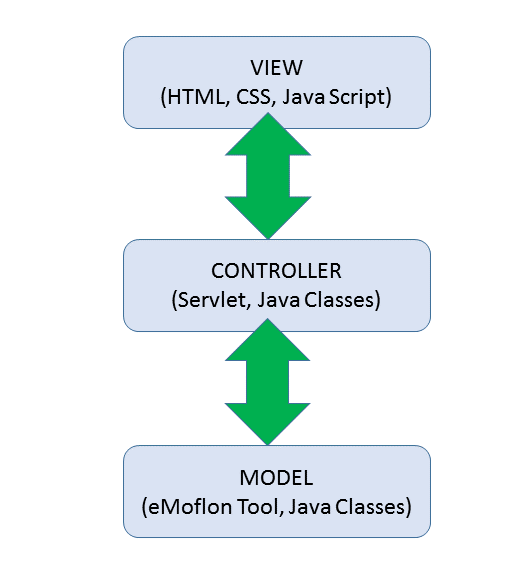
\includegraphics[width=1\textwidth]{figures/Highlevel_Arch}
	\caption{High Level Architecture Diagram}
	\label{fig:Architecture_Diagram}
\end{figure}
\subsubsection{View (GUI)}\label{subsubsec:view}
\subsubsection{Controller}\label{subsubsec:controller}
\subsubsection{Model}\label{subsubsec:model}






